\section{Design Document}

The Design Document (DD) serves various essential purposes within the software development process:
\begin{itemize}
    \item \textit{Communication}: it acts as a communication tool facilitating interaction among requirement analysts, architects, and developers. 
    \item \textit{Refinement of plan and estimations}: it allows for a more accurate assessment of the resources, time, and effort required for implementation.
    \item \textit{Baseline for implementation activities}: it outlines the design choices, architectural decisions, and key components that developers will build upon during the coding phase.
    \item \textit{Traceability}: this ensures that each requirement has a clear association with the components responsible for its implementation, aiding in project management and quality assurance.
    \item \textit{Baseline for integration and quality assurance}: in preparation for integration and quality assurance activities, the DD plays a crucial role by:
        \begin{itemize}
            \item Identifying the order of implementation, allowing for a structured and phased development approach.
            \item Defining the integration strategy, outlining how different components will be integrated into the complete system.
            \item Supporting verification and validation processes, ensuring that the developed system meets the specified requirements and quality standards.
        \end{itemize}
\end{itemize}
\begin{figure}[H]
    \centering
    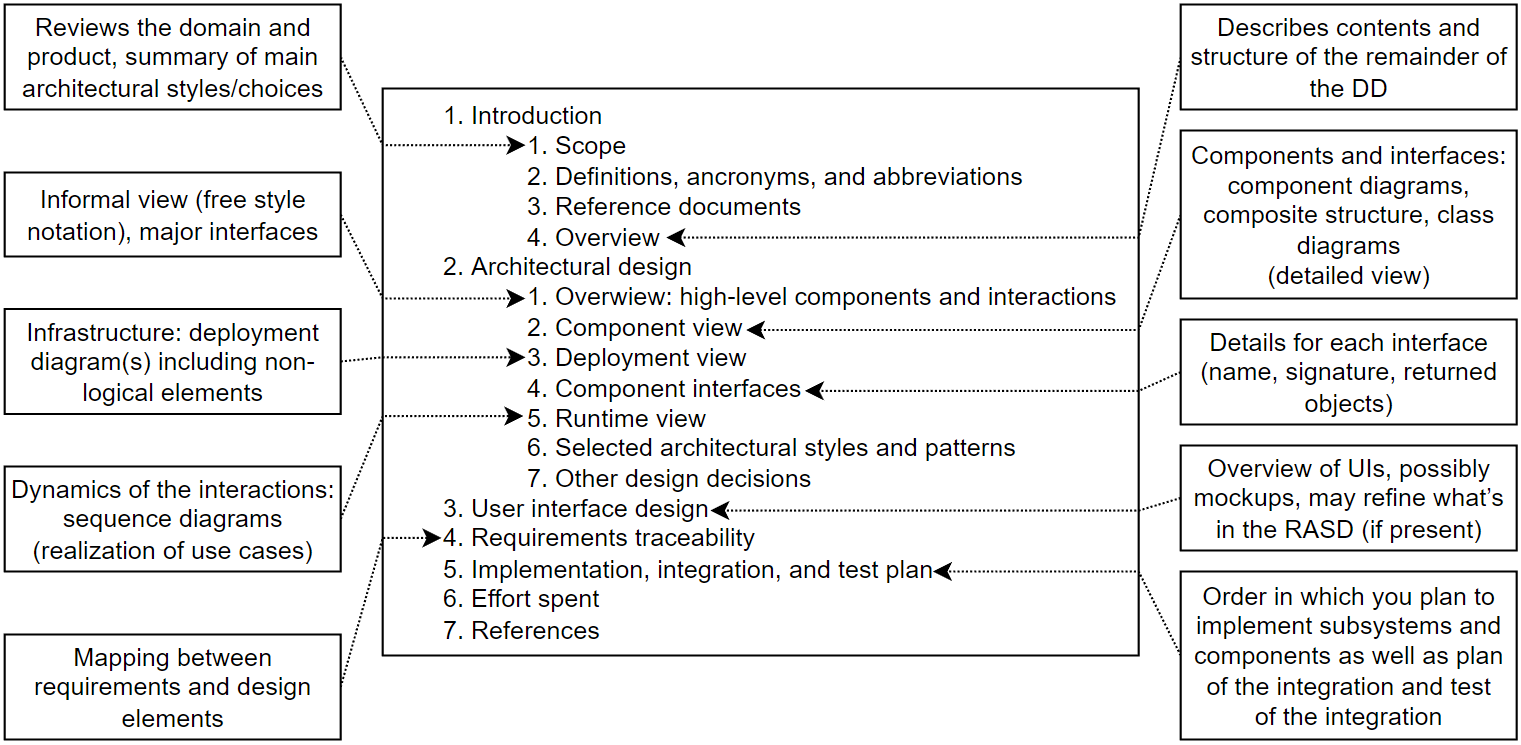
\includegraphics[width=1\linewidth]{images/dd.png}
    \caption{IEEE standard for DD}
\end{figure}